\documentclass[11pt,a4paper]{report}
\usepackage{amsmath}
\usepackage{amsfonts}
\usepackage{amssymb}
\usepackage{setspace}
% colored tables
\usepackage{color, colortbl}
%define grey color
\definecolor{Gray}{gray}{0.9}
\usepackage{fancyhdr}
% cool band at the top of each page
\usepackage[utf8]{inputenc}
\usepackage[T1]{fontenc}
% french accents support
\usepackage{titlesec}
\usepackage{textcomp}
\usepackage{gensymb}
\titleformat{\subsection}{\itshape\normalsize}{\thesubsection}{1em}{}
% interligne
\usepackage{tocloft}
% table of contents customization
\usepackage{pdflscape}
\usepackage[section]{placeins}
\usepackage[sectionbib]{natbib}
% No newpage before bibliography
\usepackage[left=2cm,
			right=2cm,
			top=3cm,
			bottom=3cm]{geometry}
            \author{Cyril Matthey-Doret}
\usepackage{outline} \usepackage{pmgraph} \usepackage[normalem]{ulem}
\usepackage{verbatim}
\pagestyle{fancy}
\setlength{\footskip}{80pt}
% chargement des figures
\setcounter{secnumdepth}{0}
% Sections will not be numbered by default
\usepackage{graphicx}					
\usepackage{wrapfig}
\usepackage[export]{adjustbox}
\usepackage[labelfont=bf]{caption}
\usepackage[colorlinks=true,citecolor=black,linkcolor=black,urlcolor=black]{hyperref}
\title{
\includegraphics[width=1.8in]{lo_unil_fbm06_bleu.pdf} \\
\vspace*{0.5in}
\textbf{Ecole de Biologie}\\
\vspace*{0.5in}
\textbf{Genetics of Sex Determination in a Parasitoid Wasp}}

\author{Travail de Maîtrise universitaire ès Sciences en Sciences moléculaires du vivant\\
		\textit{Master Thesis of Science in Molecular Life Sciences}\\
        		\vspace*{0.2in}\\
                par\\
                \vspace*{0.1in}\\
		\Large{Cyril Matthey-Doret}\\
        		\vspace*{0.2in} \\
        Director: Professor Tanja Schwander\\
        Supervisor: Doctor Casper van der Kooi\\
        Expert: Doctor Jonathan Romiguier\\
        \vspace*{0.2in}\\
		Department of Ecology and Evolution\\
        \textbf{University of Lausanne - Switzerland}\\
       } \date{\today}
%--------------------Make usable space all of page
\setlength{\oddsidemargin}{0in} \setlength{\evensidemargin}{0in}
\setlength{\topmargin}{0in}     \setlength{\headsep}{+0.5in}
\setlength{\textwidth}{6.5in}   \setlength{\textheight}{8.5in}
\setlength{\headheight}{13.6pt}
%--------------------Indentation
\setlength{\parskip}{\baselineskip}%
\setlength{\parindent}{0pt}%
\renewcommand*\contentsname{Table of contents}
% change table of contents title
\begin{document}

%--------------------Title Page
\renewcommand{\headrulewidth}{1pt}
\fancyhead[R]{Master Project, University of Lausanne - January 2018}
\maketitle
%--------------------Begin Outline

\tableofcontents
\newpage

\section{Abstract}
Sex determination has evolved in a variety of ways throughout the tree of life and can depend on environmental and genetic signals. In most species of Hymenoptera, a large order of insects comprising ants, bees and wasps, the molecular mechanism underlying sex determination is known as complementary sex determination (CSD). In species with CSD, heterozygosity at one or a few loci induces female development. Here, we identify the genomic regions underlying CSD in the parasitoid wasp \textit{Lysiphlebus fabarum} using restriction-site associated DNA sequencing (RADseq). We analyse the sex-specific segregation of polymorphic sites among 530 diploid males and females using association mapping. We report multi-locus CSD with four candidate loci, all on different chromosomes and three close to centromeric regions. None of the candidate regions feature evidence for homology with the \textit{csd} gene from \textit{Apis mellifera}, the only species in which CSD has been characterized. Our results suggest that the molecular mechanisms underlying CSD in different species can differ and are less conserved than previously thought. Moreover, no homology is shared between the candidate loci, contrasting with previous suggestions that multiple CSD loci should emerge from duplications of an ancestral locus. As CSD regions should be under balancing selection, we propose to further validate candidates from the current study by testing whether they coincide with peaks of allelic diversity in wild populations.

\section{Résumé}
La détermination du sexe a évolué de nombreuses façons à travers l'arbre de la vie et peut dépendre de signaux environnementaux et d'informations génétiques. Dans la plupart des espèces d'Hyméno\-ptères, un important ordre d'insectes comprenant les fourmis, les abeilles et les guêpes, le mécanisme moléculaire qui sous-tend la détermination du sexe est appelé détermination sexuelle complémentaire (CSD). Chez les espèces avec CSD, les individus hétérozygotes à un ou quelques loci se développent en femelles. Dans l'étude présente, nous identifions les régions génomiques responsables du CSD dans la guêpe parasitoïde \textit{Lysiphlebus fabarum} en utilisant le séquençage d'ADN assisté par site de restriction (RADseq). Nous analysons la ségrégation de sites polymorphiques entre sexes dans 530 femelles et mâles diploïdes par association génétique. Nous rapportons quatre loci CSD, tous sur différents chromosomes, et trois proches des régions centromériques. Aucune des régions candidates ne présente de signes d'homologie avec le gène \textit{csd} d'\textit{Apis mellifera}, la seule espèce dans laquelle CSD a été caractérisé. Nos résultats suggèrent que les mécanismes moléculaires responsables de CSD peuvent différer d'une espèce à l'autre et sont moins conservés que ce qui était pensé précédemment. De plus, aucune homologie n'est partagée entre les loci candidats, contrastant avec les prédictions que de multiples loci CSD pourraient émerger de dupplications d'un locus ancestral. Puisque les régions CSD devraient être sous sélection équilibrante, nous proposons de confirmer les candidats de cette étude en testant s'ils coïncident avec des pics de diversité allélique dans des populations sauvages.

\section{Introduction}
Sex determination is the crucial stage of life where the development of an organism is oriented towards male or female differentiation. Sex determination mechanisms can be based on genetic factors, environmental cues, or both \citep{Beukeboom2014EvolSexDetBook}. Genetic sex determination is most common \citep{Bachtrog2014SexIt} and can be achieved for example by sex-chromosomes or sex-specific ploidy. An active area of research in evolutionary biology focuses on the evolution and mechanisms of sex determination. Insects are a good system to investigate these fundamental questions, because they feature a wide array of sex determination systems. 

Several fields of applied research would also benefit from a better understanding of insect sex determination systems and their underlying genetics. For example, in agriculture, females of many parasitoid wasp species lay their eggs in crop pests and are used extensively in biological control \citep{lasalle1993parasitic}. Studies on sex determination can also have implications in public health. Mosquitoes, for instance, are important vectors of several diseases including malaria, but only females transmit the diseases \citep{Krzywinska67}. 

A common sex determination system in arthropods is haplodiploidy, where unfertilised eggs develop into (haploid) males, and fertilised eggs develop into (diploid) females. Haplodiploidy is one of the major sex determination systems, found in approximately 12\% of all animal species \citep{Bachtrog2014SexIt}, encompassing the insect orders Thysanoptera (thrips) and Hymenoptera, the latter being one of the largest orders of insects with around 150,000 described species \citep{Mayhew2007WhyPhylogenies} comprising wasps, bees, ants and sawflies. Although haplodiploidy is a well described phenomenon, the underlying genetic architecture linking it to sex determination is still largely unknown. In many haplodiploid species, female development depends on the heterozygosity of the complementary sex determination (CSD) gene(s) \citep{Crozier1971}. In the case of a single CSD locus (sl-CSD), the organism develops into a female when heterozygous at the CSD, or into a male if homozygous or hemizygous at the CSD. In species with multilocus CSD (ml-CSD), female development is induced if at least one of the CSD loci is heterozygous. Thus, haploid eggs develop into males, as they are hemizygous for all loci, and diploid eggs, when individuals are heterozygous for at least one CSD locus, develop into females. CSD is the best known sex determination mechanism in haplodiploids and is thought to be the ancestral system in Hymenoptera \citep{Miyakawa2015}. Thus far, evidence for the presence of CSD has been obtained in more than 60 hymenopteran species \citep{VanWilgenburg2006}; yet, the molecular pathway of CSD is described only in the honey bee \citep{Beye2003}.  In the honey bee, the \textit{csd} gene stems from a duplication of \textit{transformer}, a major sex determination player in insects \citep{Bopp2014SexTheme}. The roles of \textit{transformer} differ between clades and it was duplicated repeatedly throughout evolution \citep{Privman2013}. The honey bee \textit{csd} gene underwent strong positive selection, resulting in its neo-functionalisation. When present in a heterozygous state, it acts as the master switch for female development by splicing the transcript of its paralog, \textit{feminizer} \citep{Hasselmann2008}.

In species with CSD, a special case occurs when, for example in strongly inbred populations, low allelic diversity will result in homozygosity at the CSD locus or loci. In this case, because only one allele is present at each CSD locus, the diploid egg will develop into a male \citep{Whiting1943} . Depending on the species, diploid males are sterile, have reduced survival or fertility \citep{Holloway1999SurvivalBraconidae}, or - as in social systems - are killed \citep{Woyke1963DroneHoneybee}. When identifying the sex determination mechanism of hymenopteran species, the presence of such diploid males is usually considered a strong indicator for CSD \citep{Butcher2000Single-locusIchneumonidae}. In species with ml-CSD, the number of sex-determining loci can be estimated by measuring the increase in diploid male production over generations of inbreeding and comparing it to simulated values using mathematical models with different numbers of loci \citep{Engelstadter2011,Boer2008ExperimentalVestalis}.

The CSD gene(s) can be found by comparing genomic regions for which females are often heterozygous and diploid males are strictly homozygous. Unfortunately, in many species, diploid males are difficult to come by, as they often have reduced fitness \citep{Heimpel2008}. However, a recent study on the genetic basis of asexuality in the parasitoid wasp \textit{Lysiphlebus fabarum} (Hymenoptera: Braconidae) (van der Kooi et al., unpublished) established multiple (asexual) lines with exceptionally high rates of diploid males production. Hence, these lines provide an excellent case to study the genetic underpinnings of CSD. \textit{L. fabarum} has both sexual and asexual lineages, where CSD is known to be the mechanism underlying sex determination \citep{Engelstadter2011}. In asexual \textit{L. fabarum}, the cytological mechanism responsible for female-producing parthenogenesis (asexuality) is central-fusion automixis \citep{Belshaw2003}, in which two meiotic products originating from homologous chromosomes fuse to produce a zygote. In this form of automixis, transitions to homozygosity happen in regions distal to recombination events (Figure \ref{CFA}a), allowing to retain relatively high levels of genome-wide heterozygosity, especially if recombination rates are low \citep{Baudry2004Whole-genomeAnalysis}. Heterozygosity is expected to decrease with distance from centromeres, therefore CSD loci that are close to the centromeres should be retained more often when passing through asexual generations (Figure \ref{CFA}b). 

In this study, we explore the genetic basis of CSD in \textit{L. fabarum}. Using restriction-associated DNA sequencing (RADseq) \citep{Davey2010} and association mapping, we study the segregation of polymorphic loci to identify regions that are highly homozygous in males, and heterozygous in females. We identify 4 candidate CSD loci, all on different chromosomes and of which 3 are close to centromeric regions. 

Uncovering whether the mechanism underlying CSD in a distant species such as \textit{L. fabarum}, is similar to the honey bee (\textit{Apis mellifera}), or if a different mechanism evolved independently, will provide valuable insight into the evolution of sex determination in insects.

\section{Results}
A previous crossing experiment (van der Kooi, unpublished) generated 45 families consisting of asexual mothers with daughters and diploid sons. In total, 583 individuals were genotyped by restriction-associated DNA-sequencing (RADseq). For all analyses, we use contigs from the latest version of the \textit{L. fabarum} reference genome (Dennis et al, unpublished) which were previously anchored into 6 chromosomes (van der Kooi et al, unpublished) in line with the six chromosomes that were deduced from karyotyping \citep{Belshaw2003}. Among the 583 samples, 53 individuals with abnormally low numbers of reads mapping to the genome were excluded. We processed the sequencing data and generated a catalog of loci from the 530 remaining samples. To identify candidate CSD regions, we followed the sex-specific frequency of heterozygosity at the polymorphic loci identified through RADseq.

\subsection{Exclusion of haploid males}
Asexual females produce haploid males in addition to diploid males and females. Such (haploid) male production is common in asexuals \citep{vanderKooi2014OnAsexuality} and may occur, for instance, when central fusion fails to happen at the end of meiosis. Since our approach relies on the comparison of heterozygosity between sexes, haploid males are not informative and should be excluded. As they are morphologically identical to diploid males, it is not possible to identify them visually. Instead, to confidently classify the ploidy of all individuals, we relied on the proportion of homozygous single nucleotide polymorphisms (SNPs) in each individual. Haploids are hemizygous at all SNPs and should therefore show complete homozygosity at all loci. However, due to possible sequencing errors and paralogous merging, some loci in haploid males may be heterozygous. We first called SNPs using stringent parameters, filtering out those with less than 20X sequencing depth. 1521 high confidence SNPs passed the quality filters and on average, each sample presented 1439 of these sites with a mean coverage of 127X. The proportion of homozygous SNPs per individual forms a bimodal distribution where the most heterozygous mode contains both males and females, while the most homozygous mode contains only males (Figure \ref{ploidy}). Although we assume haploid males to be in the most homozygous peak, modes are not perfectly separated. To avoid misclassification of haploids as diploids, we used a conservative threshold, requiring a minimum of 90\% homozygous SNPs to consider a sample haploid. Using this strategy, we excluded 216 haploid males and kept 148 females and 166 males for downstream analyses.

\subsection{Identification of  CSD}
After excluding haploid males, SNP calling was performed again on the 314 diploids with a more permissive sequencing depth filter of 5X and allowed to retrieve 2630 SNPs. On average, each sample presented 2260 SNPs with a mean coverage of 80X. 

With this number of sites relative to a genome size of 170Mb, the marker density achieved makes it unlikely to identify SNPs directly inside CSD loci. Instead, we used association mapping to identify SNPs that are close to the CSD regions and segregate with it through linkage disequilibrium. To identify such SNPs, we used a case-control design where we test the association of allelic state (homozygous and heterozygous) with sex (male and female, respectively). We performed a Fisher-exact test to score every SNP based on the relative proportion of homozygous males versus females at a locus. High scoring SNPs are therefore consistently found in a heterozygous state in females and/or in a homozygous state in males. Such pattern would be expected from regions surrounding a CSD locus and affected by linkage disequilibrium. After correcting for multiple testing using the Benjamini-Hochberg method, we found 4 candidate loci ($p<10^{-3}$), all on different chromosomes (Figure \ref{assoc}), among which 2, on chromosomes 3 and 5, are highly significant ($p<10^{-4}$). 

The fit of the CSD candidates i.e. the proportion of individuals whose genotype fits the CSD model at a given site, is expected to have different strength in males and females. Since males must be homozygous at all CSD loci, we expect them to show a very strong fit at all CSD candidates. Females, on the other hand, need only be heterozygous at one of the CSD loci and should therefore show a weaker fit. Decomposing the strength of this CSD association into sex by looking separately at the proportion of heterozygous females and homozygous males revealed that the peaks on chromosomes 1 and 3 show stronger association in males, while the peak on chromosome 5 shows stronger association in females (Figure \ref{assoc}). This information therefore provides better support for the CSD role of candidates on chromosomes 1, 2 and 3 than on chromosome 5.

\subsection{Location of centromeric regions}
In central-fusion automixis, the genotype of any diploid offspring should be identical to that of their mother, except for regions distal to recombination events that can become homozygous (Figure \ref{CFA}). This causes homozygosity to increase with distance from the centromere. Thus, for loci that are heterozygous in the mother, the proportion of homozygous offspring can be used as a proxy for recombination rates. 

Regions of low recombination rates are used to estimate the position of centromeric regions. We could clearly infer the location of the centromeric regions on five out of six chromosomes (Figure \ref{centro}). Modeling recombination rates using both weighted local regression and moving averages yielded similar results (Figure \ref{centro}). For chromosome 6 which has a limited number of markers, it was impossible to make a reliable inference. Out of the four candidate CSD regions, three fall close to the estimated centromeric regions (Figure \ref{circular}). Such proximity is expected in organisms with central-fusion automixis, as CSD loci that are further from centromeres would be rendered homozygous in case of recombination \citep{Vorburger2014}.

\subsection{Collinearity across CSD regions}
Since heterozygosity at any single CSD locus is sufficient to induce female development, similar genetic features might be shared between the different candidate regions. Besides, it has been proposed repeatedly that ml-CSD could have emerged through gene duplication of an original CSD locus \citep{Schmieder2012TracingAnts,Boer2008ExperimentalVestalis}. A common approach to determine whether different regions share such similarity and arose through duplication events, is to look for collinearity. Collinearity is the conserved order of homologous genes between regions and is an extension of the concept of synteny. We used MCScanX \citep{Wang2012MCScanX:Collinearity} to investigate genome-wide patterns of collinearity in genes and transcripts. The coordinates used were generated by combining gene tracks from the MAKER annotation pipeline (Dennis et al, unpublished) and transcripts coordinates from RNAseq data in larvae \citep{Dennis2017ParasitoidHosts}. Using the union of these elements, we found no evidence for collinearity between candidate CSD regions (Figure \ref{circular}). A genuine absence of collinearity could mean either that the CSD-causing features differ across loci, or that the similar region is not large enough to be detected using collinearity. It is also possible that the assembly is too fragmented to detect collinearity. The genome is indeed split into 1698 contigs (Table \ref{genome}) of which 296, accounting for 53.5\% of the assembly length, were anchored into chromosomes using a linkage map (Table \ref{anchored}). It is therefore possible, that missing unanchored contigs are interrupting collinearity blocks inside chromosomes.

\subsection{Transformer homology}
To investigate whether \textit{transformer}, the homolog of the honey bee \textit{csd} and \textit{feminizer} genes, is present in the candidate CSD regions, we retrieved the protein sequences of \textit{feminizer} orthologs from 8 different Hymenopteran species and searched \textit{L. fabarum} genome for them using TBLASTN. A strong homology is present in chromosome 1 at 7Mb (positions: 7,006,657-7,006,839), however there is no CSD candidate in that region. There was not any hit in the unanchored contigs either, which would suggest none of the CSD candidate regions contain a \textit{transformer} homolog.

\section{Discussion}
We identified ml-CSD in the parasitoid wasp \textit{Lysiphlebus fabarum} and found four candidate regions, all on different chromosomes. The candidate locus on chromosome 3 is supported by the most sites and shows the most significant association. 

Previous studies suggested the presence of ml-CSD in this species based on diploid male proportions among offspring \citep{Engelstadter2011}. Besides, ml-CSD should be favored in species with asexual reproduction or high inbreeding, where it would decrease the load caused by diploid male production \citep{Vorburger2014}. In \textit{L. fabarum,} homozygosity generated by central-fusion could favor the emergence of multiple CSD loci in centromeric regions, where transitions to homozygosity are the least frequent. In agreement with this hypothesis, all putative CSD loci we identify, except one on chromosome 2,  are found close to centromeric regions.

To some extent, our results conflict with the canonical CSD model. This model assumes that all loci have identical effect and must all be homozygous in males, hence the expected stronger fit in males \citep{Crozier1971}. Contrastingly, the locus we identify on chromosome 5 shows a stronger association among females. There are at least 3 possible explanations for this discrepancy. First, this locus is only supported by 2 SNPs and might be a statistical false positive. Second, it could contain genetic features unrelated to CSD, but potentially lethal to females when present in a homozygous state, while having no particular effect on males. Finally, in case the locus is a true positive for CSD, we need to reconsider the ml-CSD model. The strong variations in significance across candidate loci, together with the sex-specific effect could be indicative of a more complex sex-determination system where the different loci have epistatic interactions or different regulatory roles. For example, the loci on chromosomes 2 and 5 are often found heterozygous in males and might have a weaker effect where heterozygosity at either locus would not be sufficient to induce female development. As the current analysis relies solely on heterozygosity, it is not sufficient to identify such complex interactions between loci. 

There is currently no clearly supported hypothesis for the functioning of ml-CSD. It is generally thought to originate by duplication of sl-CSD  \citep{Boer2008ExperimentalVestalis,VanWilgenburg2006}, but if the loci are truly equivalent, the model does not currently explain why a homozygous CSD would not be able to complement another one by acting as a second allele. In the light of our results, it seems more likely that the different CSD loci function differently. The lack of collinearity between loci would also support that ml-CSD differ and did not arise from duplication. Nevertheless, a technical artifact caused by the high number of unanchored contigs cannot be fully excluded. It would be worth improving the placement of contigs by producing a new linkage map with more markers, or directly improving the assembly. Such analysis would allow retrieving more complete CSD regions and might confirm whether they really show no collinearity, or if absence of collinearity is simply due to missing segments. Nonetheless, the association mapping step is not affected by genome completeness and the pattern we observe lays the foundations for more detailed investigation of the CSD regions.  

In a recent study, ml-CSD was identified in the ant \textit{Vollenhovia emeryi} for the first time using genomics. The two CSD loci identified did not share any homology \citep{Miyakawa2015}. This finding would also support different roles of the sex determining loci in ml-CSD. Among the two loci reported in \textit{V. emeryi}, one featured two homologs of the \textit{transformer} gene, the ortholog of the honeybee \textit{csd}, while the second shared no identity \citep{Miyakawa2015}. Unlike in \textit{V. emeryi}, where it would appear the CSD mechanism is at least partially similar to the honey bee, \textit{L. fabarum} seems to offer a completely novel mechanism which does not rely on \textit{transformer}.

Finally, it is important to outline that we are using a single laboratory strain and there could be more CSD regions in wild populations of the species that were fixed to homozygosity in the asexual females used in the current study. Nonetheless, among the CSD regions we detect, we can conclude there is no \textit{transformer} homolog, since neither CSD regions nor unplaced contigs show such homology. That is clear evidence that \textit{L. fabarum} CSD could be caused by another mechanism than that of the bee. This is reinforced by the absence of collinearity among loci, as a \textit{transformer}-based ml-CSD system would likely rely on duplications of an original region, thus maintaining collinearity. There are currently two known genetic mechanisms underlying  haplodiploid sex determination in Hymenoptera \citep{VanDeZande2014GenomicDetermination}: sl-CSD, in the honey bee \textit{Apis mellifera}, and maternal genome imprinting, in the jewel wasp \textit{Nasonia vitripennis} \citep{Beukeboom2010}. Functional investigation of the CSD regions presently identified could potentially uncover a third, novel molecular mechanism of sex determination in Hymenoptera.

A possible approach to validate the candidate loci we identify would be to measure allelic diversity along the genome of wild individuals. Because diploid males (i.e. CSD-homozygous) have reduced fitness, rare CSD alleles should be positively selected in the wild \citep{Hasselmann2004SignaturesBee., Gloag2016}. Regions undergoing such balancing selection could be detected by measuring nucleotidic diversity throughout the genome. Overlap between highly variable regions and candidate CSD loci would provide an independent line of validation. 

\section{Materials and methods}

\subsection{Samples and RADseq protocol}
\textit{Performed prior to master project.}\\
A haploid male coming from an asexual family of \textit{Lysiphlebus fabarum} was crossed with two females from a highly inbred, iso-female sexual line (van der Kooi, unpublished). Following a crossing design similar to that used in \citet{Sandrock2011}, asexual females were obtained in the F3 generation. In total, 583 individuals from 45 families are used in the current study, including 11 F3 mothers, 165 F4 daughters and 407 F4 sons. The samples were kept in ethanol at -20\degree C. Males and females were distinguished phenotypically and prepared in 6 separate libraries, following the protocol from \citet{Parchman2012Genome-widePine}. ddRADseq was performed on all samples using EcoRI and MseI restriction enzymes, and fragments  of 200-450 bp were size-selected on agarose gel. Single-end sequencing was performed using Illumina Hiseq 2500. Samples were multiplexed in each library following the TruSeq multiplexing design, and libraries were pooled by pairs on the same Illumina lane using adapters iA06 or iA12.

\subsection{Genome assembly}
\textit{Performed prior to master project.}\\
The latest genome assembly (Table \ref{genome}) was provided by Alice Dennis (Dennis et al, unpublished). The contigs of this assembly were placed and ordered into chromosomes (Table \ref{anchored}) using a linkage map (Bast, unpublished) consisting of 1092 markers across 123 individuals from a single (sexual) family, and only contigs that were successfully placed into chromosomes (van der Kooi, unpublished) were used in all analyses, accounting for 53\% of the total assembly length.

\subsection{STACKS pipeline}
We used the \href{http://catchenlab.life.illinois.edu/stacks/}{STACKS} software (version 1.46) \citep{Catchen2013StacksGenomics} to process RADseq data. Following quality control using \href{https://www.bioinformatics.babraham.ac.uk/projects/fastqc/}{fastqc} (https://www.bioinformatics.babraham.ac.uk/projects/fastqc, version 0.11), the raw reads were trimmed and demultiplexed using the "process radtags" module from the STACKS suite and 2 mismatches were allowed to detect adapters. The 93bp trimmed, demultiplexed reads were mapped to the latest assembly of the \textit{L. fabarum} genome using \href{http://bio-bwa.sourceforge.net/}{BWA-aln} (version 0.7.2) \citep{Li2009} with 4 mismatches allowed. Only uniquely mapped reads were extracted using \href{http://www.htslib.org/}{samtools} (version 1.3) \citep{Li2009TheSAMtools}. Stacks were then generated from SAM files of unique hits using the Pstacks module, requiring a minimum read depth (-m) of 3 to consider a stack. Individuals with less than 10\% uniquely mapped reads compared to the average of all samples were excluded from the analysis. The catalog of loci was built with Cstacks allowing for a distance (-n) of 3 mismatches between samples at each locus. Populations was run on all samples together, requiring each locus to be present (-r) in at least 80\% of samples and have at least a sequencing depth (-m) of 20 for ploidy separation, or 5 for association mapping (Table \ref{RAD_stats}). The different STACKS parameters were selected following guidelines in \citet{Paris2016}.

\subsection{Ploidy separation}
To determine the ploidy of all individuals, we rely on genome-wide homozygosity levels. Haploid samples should have extremely high homozygosity levels compared to diploid ones. We called only high confidence SNPs in STACKS populations module by using a stringent cutoff of 20 reads for the minimum sequencing depth (-m parameter). We then computed the proportion of homozygous SNPs per individual using \href{https://vcftools.github.io}{VCFtools} (version 0.1.13) \citep{Danecek2011TheVCFtools} on the output VCF file from populations. A conservative threshold of 90\% homozygosity among polymorphic sites was determined empirically based on the bimodal distribution of homozygosity. Individuals above that threshold were considered haploid and excluded from the subsequent populations run used the main analyses.

\subsection{Filtering merged paralogs}
When different regions in the genome show very high similarity, as in the case of paralog genes, the different regions might be merged into two different alleles of the same locus in the catalog. Haploid males were used to identify these "paralog merging" events. As all SNPs in these samples should have a single allele (i.e. they are hemizygous), we can single out SNPs that are recurrently heterozygous in haploids and identify them as paralog merging events. We extracted loci that were homozygous in more than 50\% of haploid samples and blacklisted them from diploid samples. This was done by rerunning populations only on diploids and specifying the list of loci heterozygous in haploids using the blacklist  (-B) parameter. In total, we blacklisted 5 loci imputed to paralog merging events from the analysis.

\subsection{Association mapping}
Both fixed and variant sites were extracted using the --genomic parameter of the populations STACKS module. Case-control association mapping was used to score CSD-candidate SNPs based on their segregation pattern. The number of heterozygous males, heterozygous females, homozygous males and homozygous females was computed for every SNP and a one-sided Fisher exact-test was performed on the 2X2 contingency table. The alternative hypothesis was that the proportion of homozygous males at the SNP is higher than the proportion of homozygous females. P-values were corrected for multiple-testing using Benjamini-Hochberg correction. 


\subsection{Centromeres identification}
The proportion of recombinant offspring along the genome was used to estimate centromere position. In each family, all sites that are heterozygous in the mother were used. If the mother was not available, a site was considered heterozygous if at least one of her offspring was heterozygous. At each site, the proportion of recombinant (homozygous) offspring was computed among all offspring whose mother was heterozygous. The proportions were then used to visualise recombination rates along the genome using two different methods: 1) computing mean homozygosity in a sliding window containing 30 sites with a step size of 1 and 2) using a weighted local regression model of degree 2 with a span of 0.6 to obtain a smooth estimate curve. The weights given to each site in the local regression correspond to the number of offspring taken into account when computing the proportion of homozygous offspring. In each chromosome, the minimum value of the local regression curve was used to approximate centromere location.

\subsection{Collinearity analyses}
Collinear blocks were defined using the default parameters of MCScanX: A collinearity block is called if two genomic segment share 5 homologous genes in conserved order with at most other 25 genes inserted in between. Gene coordinates were defined by merging maker gene prediction tracks and transcripts assembled from reference-aligned RNAseq reads from 5-days old larvae provided by Alice Dennis \citep{Dennis2017ParasitoidHosts}. Gene sequences were extracted at the merged coordinates using bedtools2 \citep{Quinlan2010BEDTools:Features} and homologous genes were defined by all versus all blastn, using the blast+ command line tools \citep{Camacho2009BLAST+:Applications}, selecting matches with an e-value inferior to 10e-05.

\subsection{Transformer homology}
Protein sequences of \textit{feminizer} orthologs were retrieved from UniproKB for 8 species of Hymenoptera: \textit{Nasonia vitripennis} \href{http://www.uniprot.org/uniprot/B3VN92}{(B3VN92)}, \textit{Euglossa hemichlora} \href{http://www.uniprot.org/uniprot/D9MZ89/}{(D9MZ89)}, \textit{Bombus terrestris} \href{http://www.uniprot.org/uniprot/B4Y115}{(B4Y115)}, \textit{Melipona compressipes} \href{http://www.uniprot.org/uniprot/B4XU23}{(B4XU23)}, \textit{Apis florea} \href{whttp://ww.uniprot.org/uniprot/A0A0H4URN0}{(A0A0H4URN0)}, \textit{Apis cerana} \href{http://www.uniprot.org/uniprot/B1NW84}{(B1NW84)}, \textit{Apis mellifera} \href{http://www.uniprot.org/uniprot/Q6V5L4}{(Q6V5L4)}, \textit{Apis dorsata} \href{http://www.uniprot.org/uniprot/B1NW85}{(B1NW85)}. Homology with these sequences was searched using TBLASTN against the \textit{L. fabarum} genome.

\section{Acknowledgements}
I wish to thank Jens Bast for generating the linkage map used to anchor contigs to chromosomes and Alice B. Dennis for providing the original assembly and the RNA-seq data. I am also thankful to Daniel L. Jeffries for helpful comments and discussions concerning RADseq and STACKS. Finally, I wish to express my sincere gratitude to Casper J. van der Kooi for his support and help throughout the project, as well as Professor Tanja Schwander who was always able to spare time to discuss and provide precious advice and suggestions.

All computations were performed at the Vital-IT (http://www.vital-it.ch) Center for high-performance computing of the SIB Swiss Institute of Bioinformatics.

\section{Figures, tables and legends}

\begin{figure}[!ht]
  \centering
  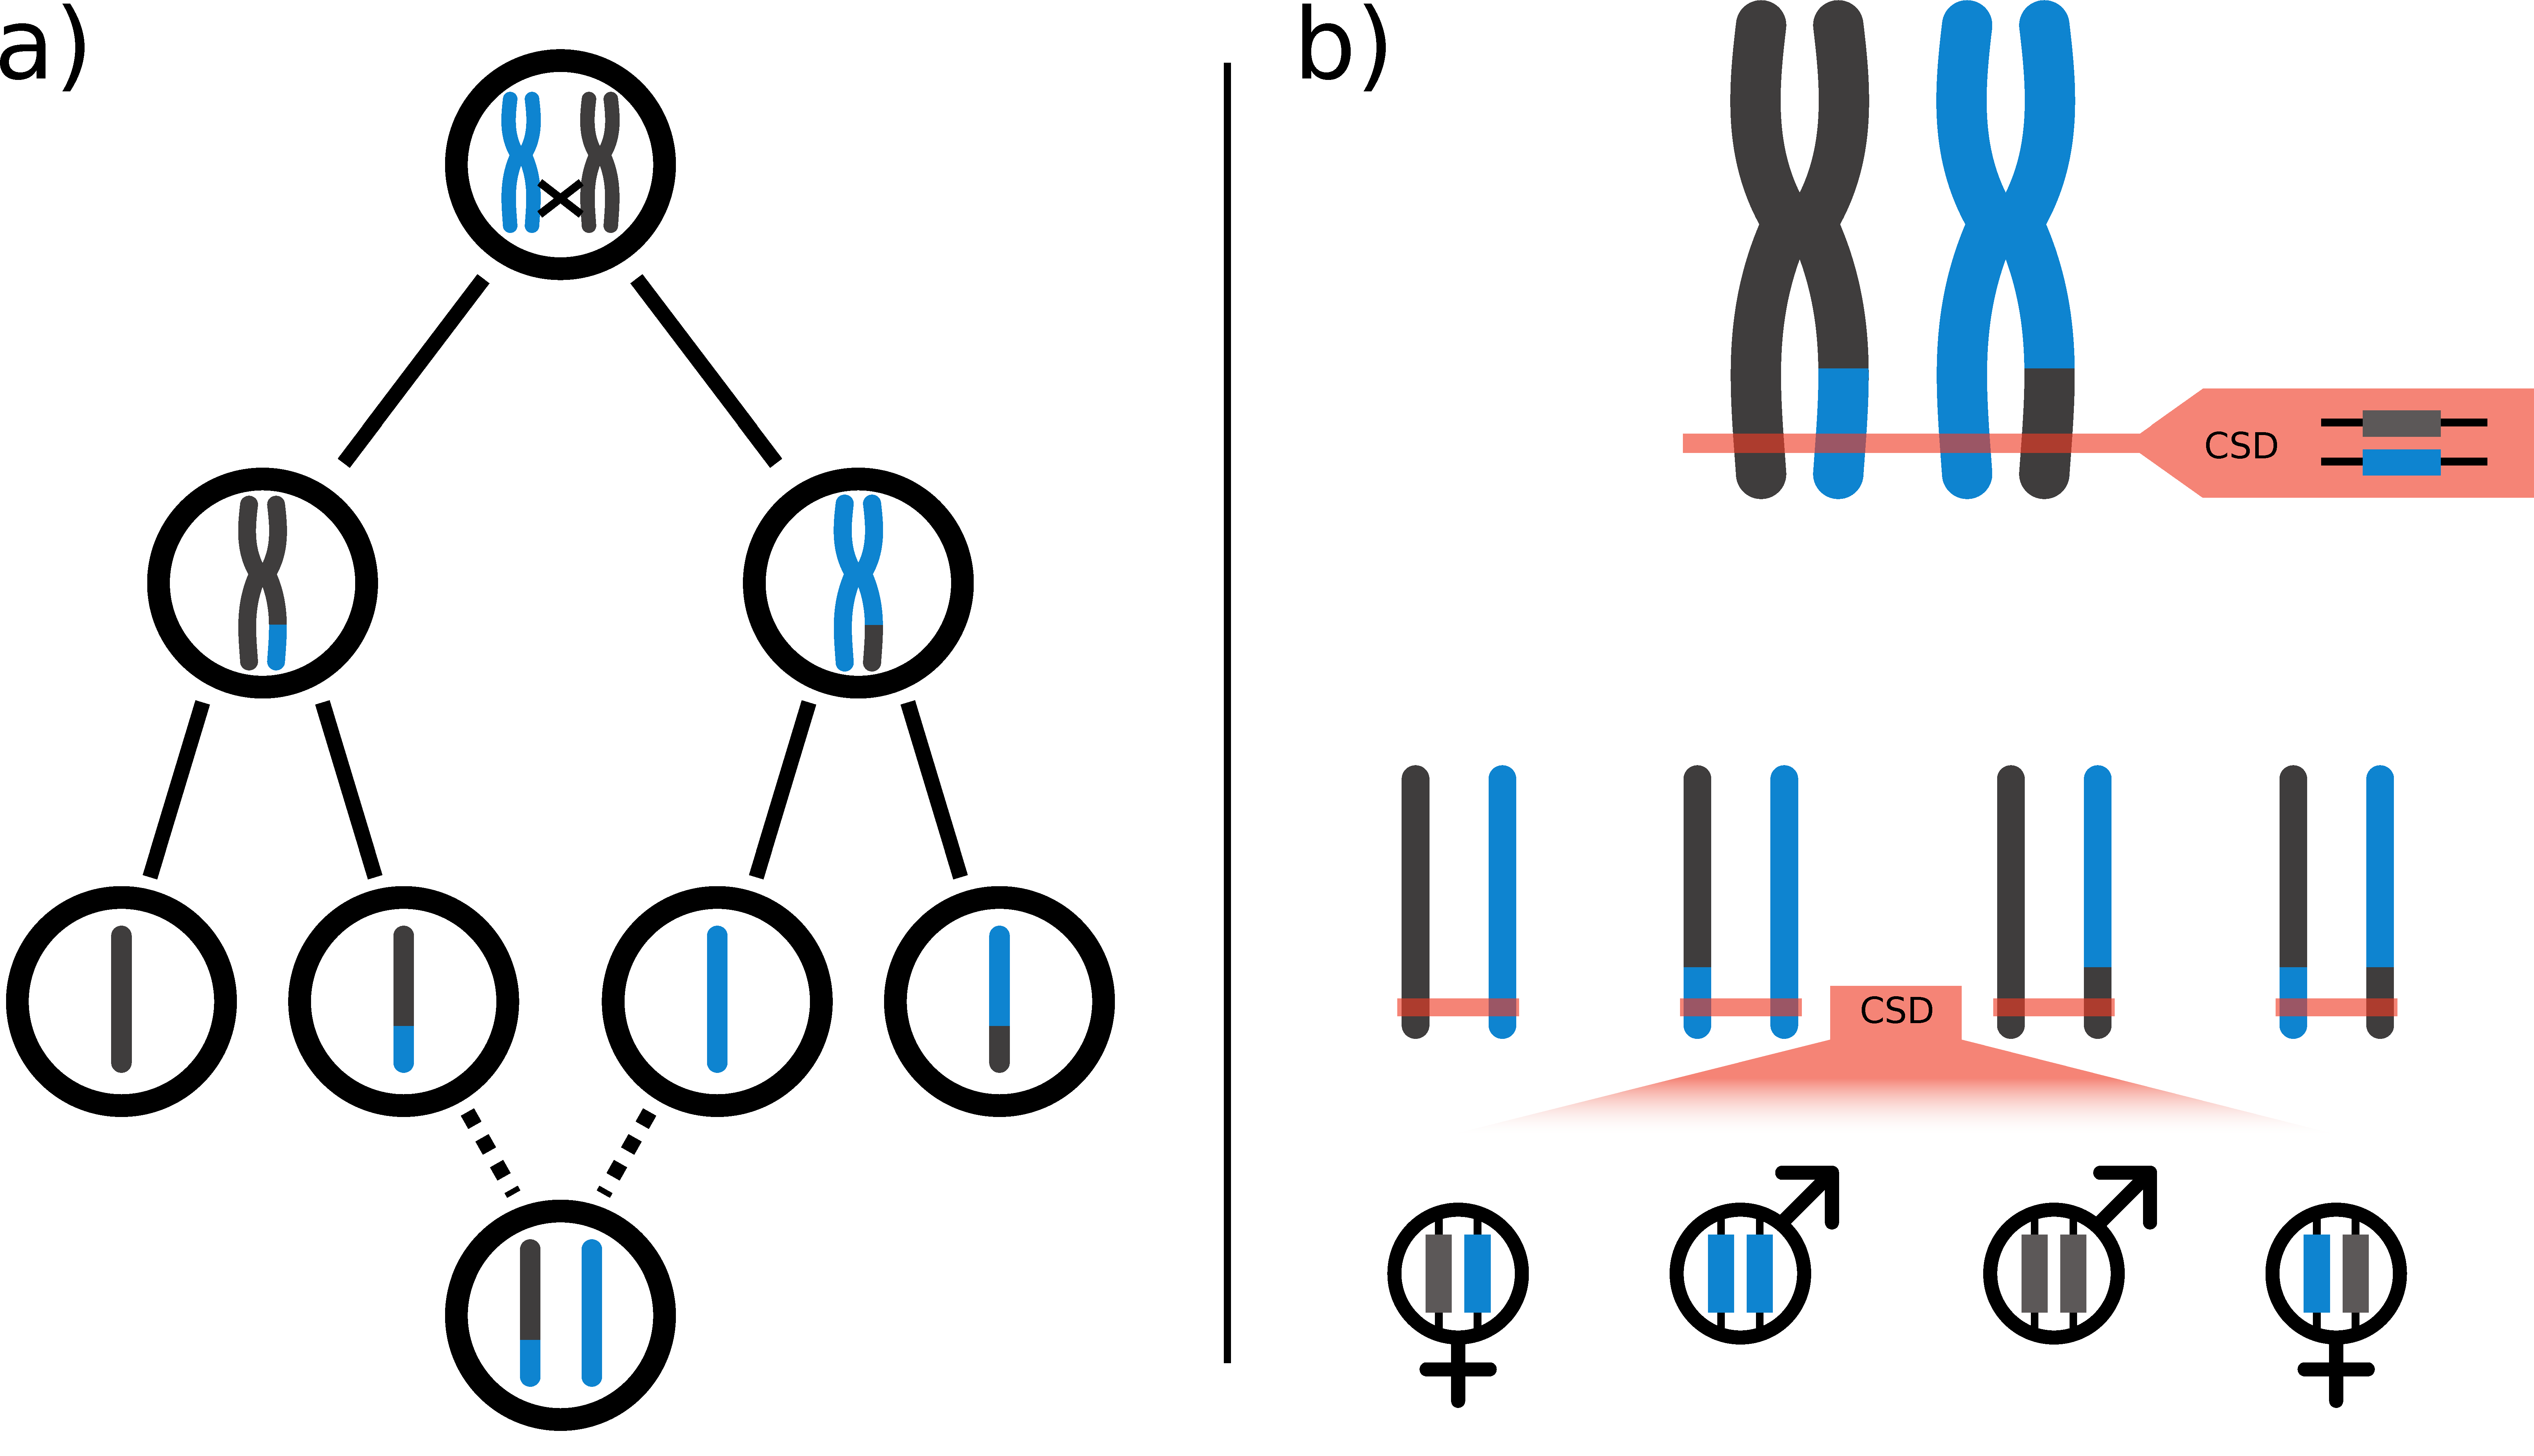
\includegraphics[width=0.8\textwidth]{figures/CFA_CSD_simple.png}
  \caption{\textbf{Central fusion automixis and CSD}. a) Meiosis under central fusion automixis with crossing over. Homologous chromosomes from the mother are represented in grey and blue respectively. The oocyte undergoes normal meiosis, until two meiotic products originating from homologous chromosomes fuse into a diploid egg. Chromosomal regions distal to a recombination event can become homozygous. b) Interaction between central-fusion and CSD. Visual representation of possible CSD genotypes in the case of a single CSD locus distal to a recombination event. If a recombination happened between the centromere and the CSD locus, an egg produced by central-fusion has 50\% chances to develop into a diploid male.}
  \label{CFA}
\end{figure}

\begin{figure}[!ht]
  \centering
  \includegraphics[width=1\textwidth]{figures/ploidy.pdf}
  \caption{\textbf{Ploidy classification.} Distribution of the genome-wide proportion of homozygous SNPs per individual. Males are represented in blue and females in red. The ploidy classification threshold of 90\% homozygosity is shown with a vertical dashed line. Individuals above this value are considered haploid.}
  \label{ploidy}
\end{figure}

\begin{figure}[!htb]
  \centering
  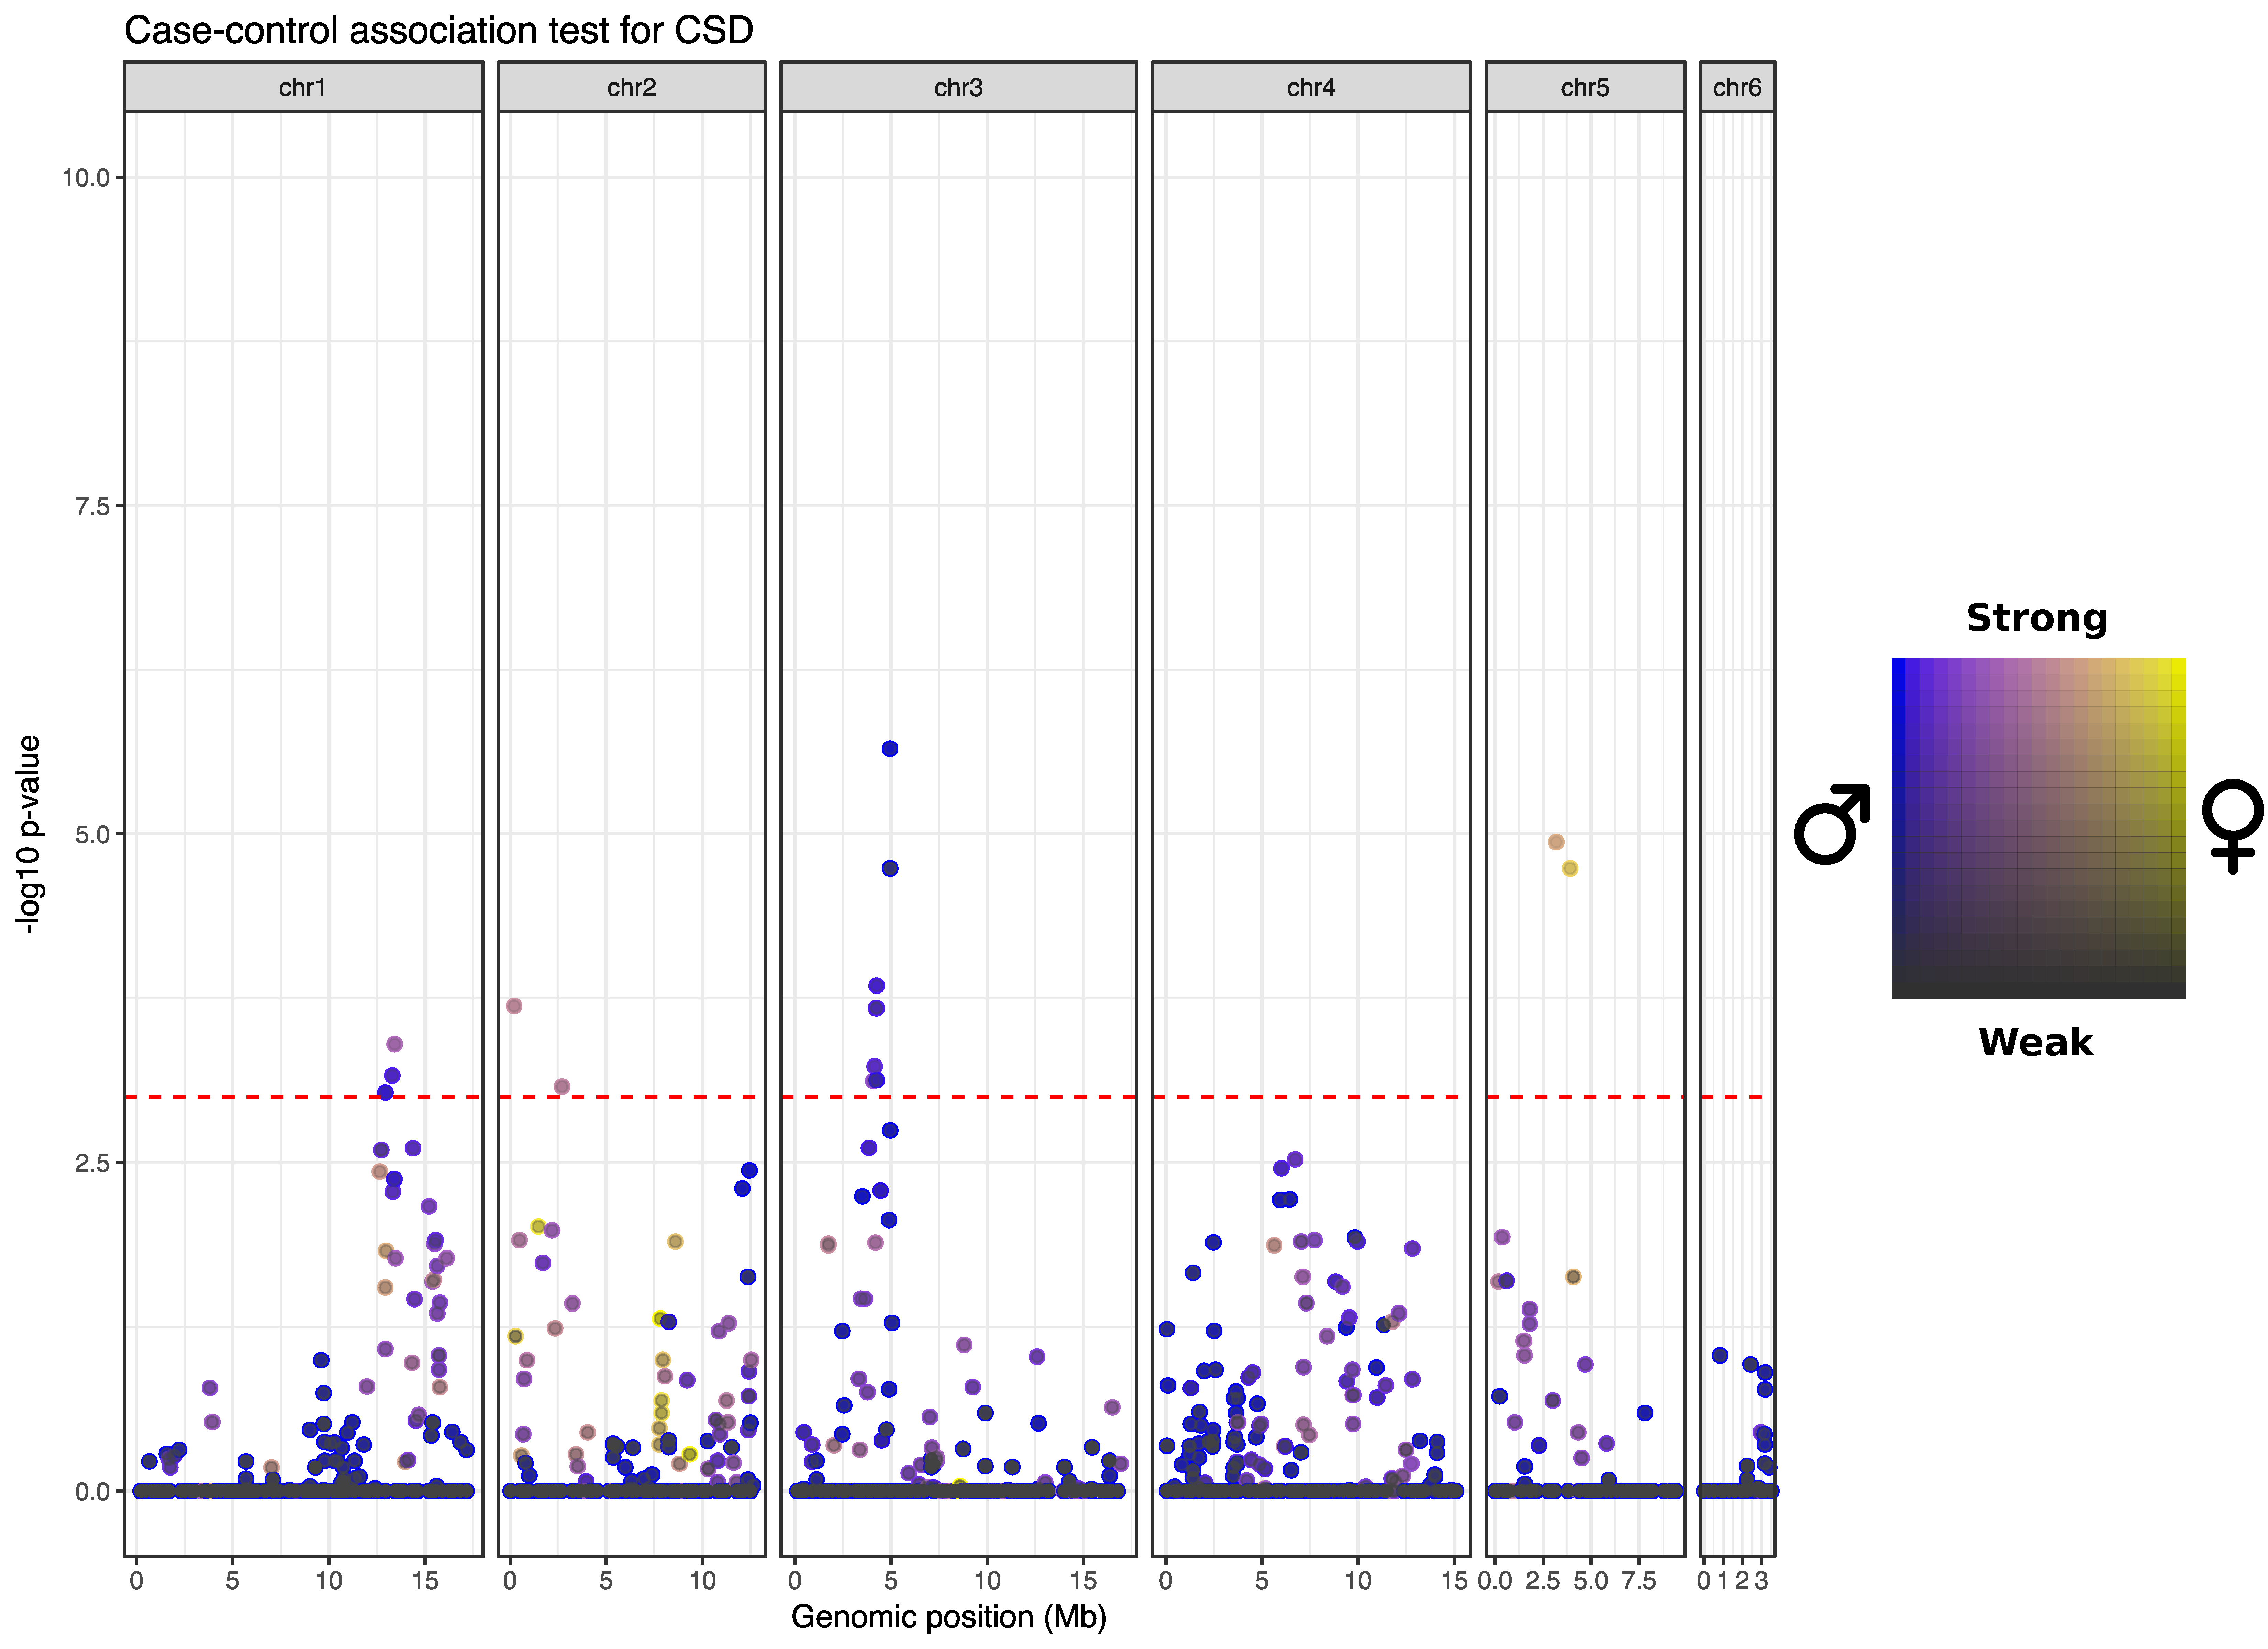
\includegraphics[width=1\textwidth]{figures/assoc_colmap_final.png}
  \caption{\textbf{\textit{L. fabarum} has ml-CSD.} Association mapping using one-sided Fisher exact test for higher proportion of heterozygous females compared to males was performed on each SNP. Manhattan plot shows -log10 p-values after Benjamini-Hochberg correction for multiple testing. Each of the 6 frames represents a chromosome, with the horizontal red dashed line showing the p = 0.001 threshold. Data points are colored according to the relative proportion of males over females whose genotype fit the CSD expectations at each SNP: At yellow points, the fit is (>2X) stronger in females, while at blue points, it is (>2X) stronger in males.}
  \label{assoc}
\end{figure}

\begin{figure}[!ht]
  \centering
  \includegraphics[width=1\textwidth]{figures/weighted_centro_final.pdf}
  \caption{\textbf{Estimation of centromeres location.} Modeling the positions of centromeres from recombination rates along chromosomes using two independent methods: Weighted local regression of degree 2 and span 0.6 (red) and a moving average with a window size of 30 SNPs and a step size of 1 (blue). 95\% confidence interval of the local regression is shown in light red. Proportion of homozygous (recombinant) offspring at each SNP is displayed as a grey dot, with area proportional to the number of individuals used to compute the proportion. Each of the 6 frames represents a chromosome and the vertical dashed lines are the centromeres, inferred as the region with lowest recombination rate along the chromosome.}
  \label{centro}
\end{figure}

\begin{figure}[!ht]
  \centering
  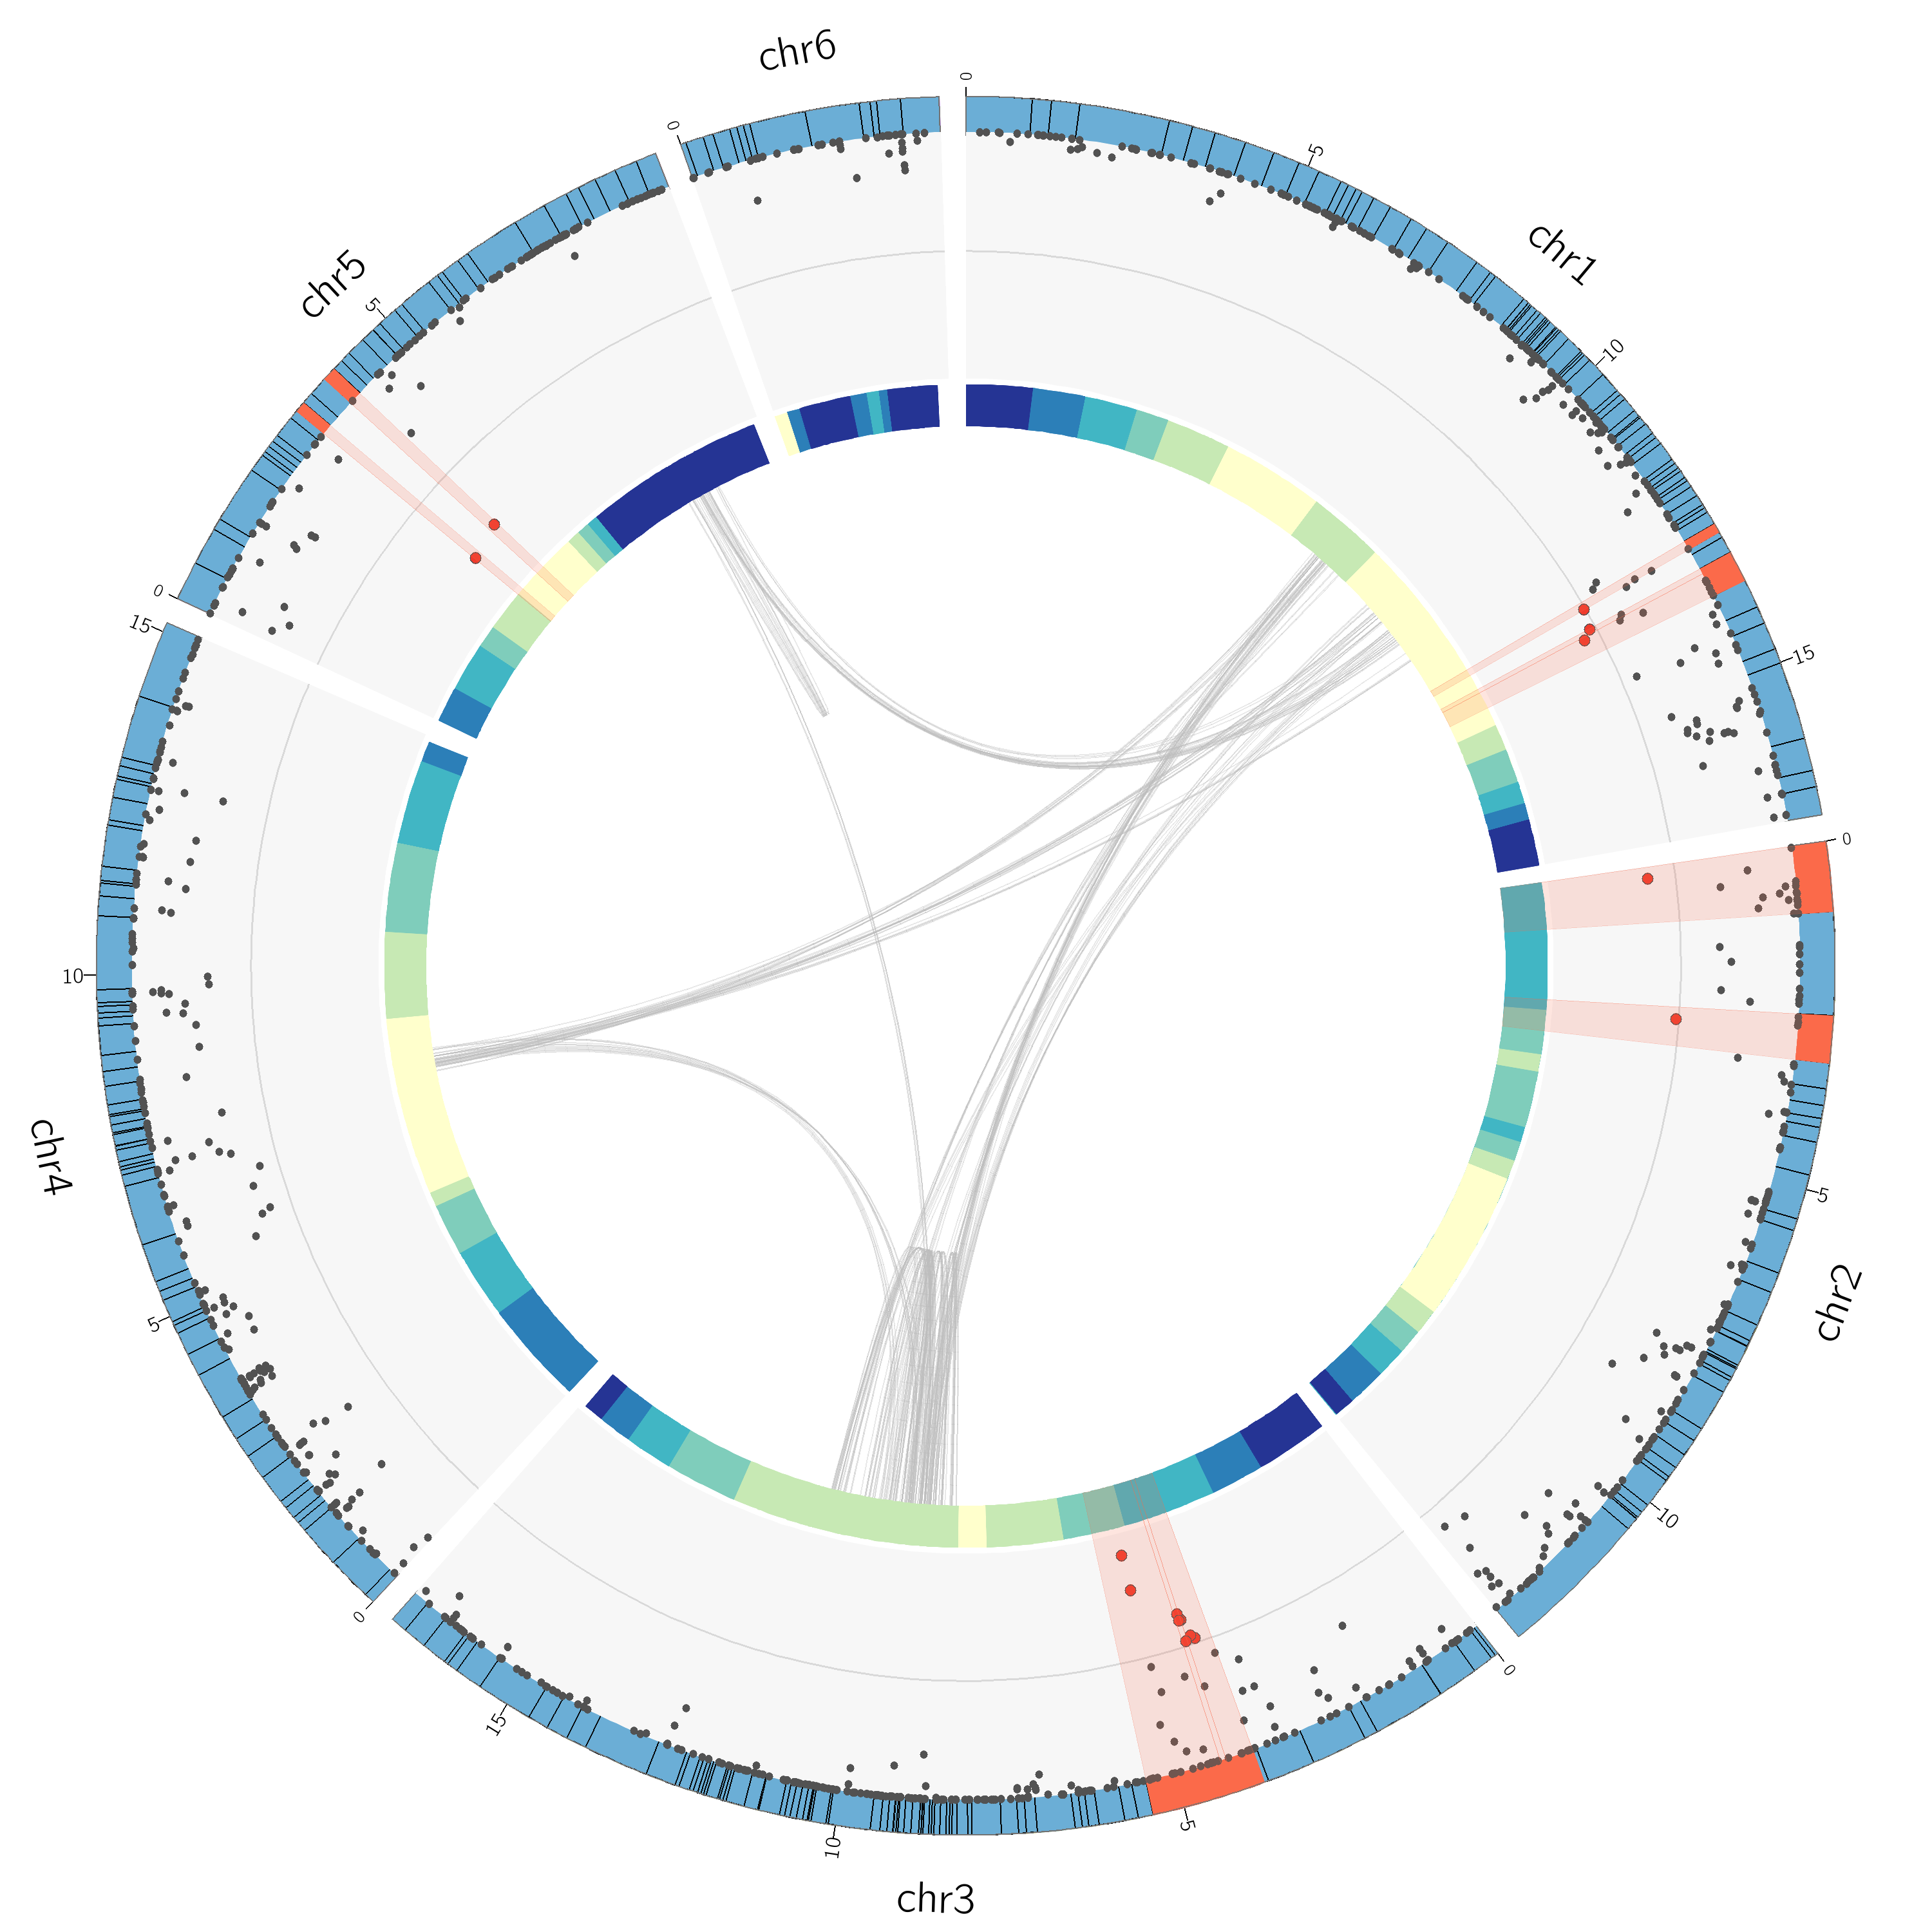
\includegraphics[width=1\textwidth]{figures/circos_col.png}
  \caption{\textbf{Position of CSD candidate regions relative to centromeres and collinearity blocks.} This plot integrates three layers of information from the current study. Each blue segment forming the outer circle represents a chromosome and the black lines intersecting them illustrate the boundaries of anchored contigs. The scatterplot shows the Manhattan plot from figure \ref{assoc} with highly significant (p < 0.001, grey line) SNPs  and their contigs shown in red. The inner colored circle is a heatmap showing recombination rate along chromosomes from low (yellow) to high (blue), estimated from proportion of recombinant offspring (Figure \ref{centro}). Bezier curves in the middle show collinearity blocks obtained using MCScanX with default parameters.}
  \label{circular}
\end{figure}

\begin{table}[!ht]
\begin{center}
\begin{tabular}{ |c|c|c|c|c| } 
 \hline
 \rowcolor{Gray}
 SNP calling run & min depth (-m) & prop. of samples (-r) & N SNPs & Mean sequencing depth\\ 
 \hline
 Ploidy classification & 20 & 80\% & 1521 & 127X\\ 
 Association mapping & 5 & 80\% & 2630 & 80X\\ 
 \hline
\end{tabular}
\end{center}
\caption{\textbf{Summary table of SNP calling statistics.} The values for STACKS populations filters for minimum sequencing depth (-m) and proportion of samples in which the locus must be present (-r) are shown for both SNP calling steps, along with the output results: Number of SNPs passing the filters, along with mean coverage per individual.}
\label{RAD_stats}
\end{table}

\begin{table}[!ht]
\begin{center}
\begin{tabular}{ l l} 
 \hline
Assembly length & 140.7 Mb\\ 
Longest contig & 2.2 Mb\\ 
Mean contig length & 82.9 kb\\ 
Median contigs length & 30.4 kb\\ 
N50 & 216.1 kb\\
Number of contigs & 1698\\ 
 \hline
\end{tabular}
\end{center}
\caption{Original assembly statistics for the \textit{L. fabarum} genome. Produced and provided by Alice Dennis (unpublished).}
\label{genome}
\end{table}

\begin{table}[!ht]
\begin{center}
\begin{tabular}{ l l} 
 \hline
Assembly length & 140.7 Mb\\
Anchored bases & 75.3 Mb\\
Anchored contigs & 296\\
Oriented contigs & 73\\
Unplaced contigs & 1402\\
N50 & 9.5 Mb\\
 \hline
\end{tabular}
\end{center}
\caption{Anchored assembly statistics. The assembly from the \textit{L. fabarum} genome in table \ref{genome} was anchored using a linkage map produced from 123 individuals and 1092 markers (Bast, unpublished). Contigs were anchored into 6 linkage groups  (van der Kooi, unpublished) representing the chromosomes according to karyotypes.}
\label{anchored}
\end{table}

\section{Supplementary Material}

Code  hosted at: \url{https://github.com/cmdoret/CSD_Lfabarum}\\

\bibliographystyle{apalike}
\fancyhead[L]{\slshape }
\bibliography{master_bib_formatted.bib}
\end{document}
